\section{Design del sistema}
In questa fase viene analizzato il software sviluppato, dando importanza all'architettura del progetto, le tecnologie utilizzate e i motivi per cui le abbiamo utilizzate, i diagrammi delle classi ed i diagrammi di sequenza dei punti scelti dal team.
\subsection{Analisi architetturale}
Questo progetto è basato sull'architettura \textbf{client-server}, è l'architettura più semplice, basata su un server ed un numero arbitrario di client. In quest'architettura i client conoscono tutti i dettagli del server (i servizi), si connettono ad esso e mandando delle richieste (HTTP), sono strettamente dipendenti da esso, infatti, in caso di modifica al server, necessitano di essere ricompilati, mentre il server risponde solo alle richieste che gli arrivano, non curandosi del tipo di client che le invia. 
\begin{figure}[H]
  \centering
  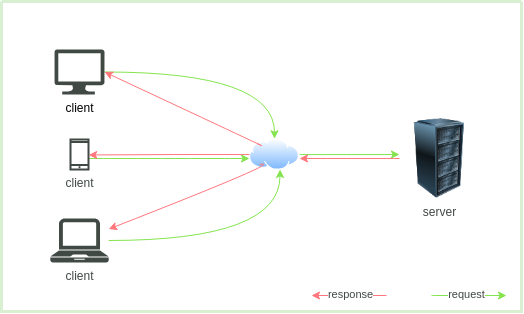
\includegraphics[scale=0.8]{img/architectureDesign/Architecture.png}
  \caption{Architettura client-server}
\end{figure}
Questo garantisce diversi vantaggi:
\begin{itemize}
  \item \textbf{Scalabilità:} Dato che il server non distingue i client richiedenti, siamo in grado, qualora fosse necessario, di scalare il server in modo da accomodare un numero maggiore (o minore) di richieste, permettendoci di risparmiare soldi e risorse.
  \item \textbf{Maggior sicurezza:} Visto che le informazioni critiche, sono archiviate solo sul server, possono essere protette meglio dalle minacce esterne con un maggiore livello di sicurezza.
  \item \textbf{Aggiornamenti} Avendo il server distaccato dai client, è possibile aggiungere nuove funzionalità ad esso, senza dover interrompere le normali operazioni di altri dispositivi.
\end{itemize}
\newpage
\paragraph{Architettura cloud}
Per garantire una fruibilità maggiore ai client, abbiamo deciso di utilizzare tecnologie cloud, questo ci permette di "potenziare" i vantaggi sopracitati, grazie alle tecnologie utilizzate dalla parte cloud.
\begin{figure}[H]
  \centering
  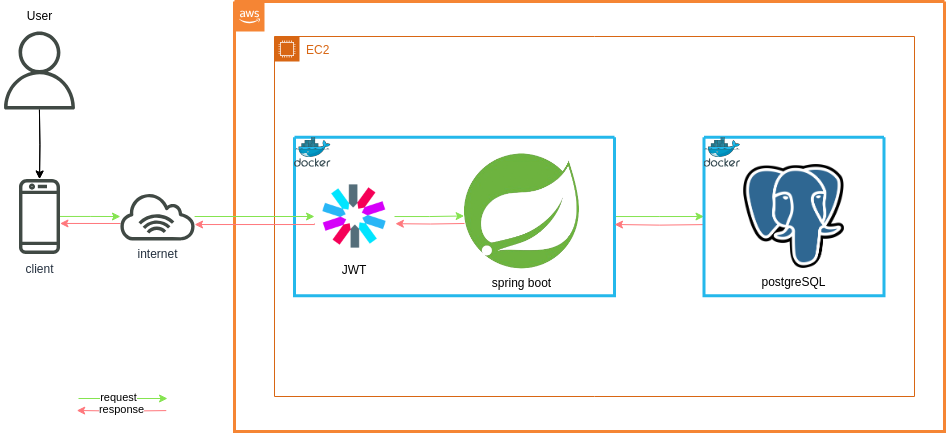
\includegraphics[scale=0.45]{img/architectureDesign/AWS.png}
  \caption{Architettura cloud}
\end{figure}
Nel nostro caso, abbiamo deciso di suddividiere la parte back-end in docker separati (postgreSQL, springboot), su macchina \textbf{EC2} fornita da \textbf{AWS}, questo ci permette di avere un sistema nel complesso più modulare e scalabile, garantendo anche la possibilità di avere aggiornamenti futuri, senza stravolgere l'esperienza dell'utente. 
\newpage
\subsection{Tecnologie utilizzate}
Le tecnologie utilizzate per lo sviluppo di questo progetto sono molteplici, divise in:\\
 progettazione, sviluppo, sviluppo della documentazione e testing.
\subsubsection{Progettazione}
\paragraph{Figma} per la progettazione dell'interfaccia grafica, lo sviluppo delle personas e la creazione del brand, ci siamo affidati a figma. Figma è un tool gratuito per la progettazione di interfacce e prototipi, può essere utilizzato sia per la progettazioni di interfacce mobile che web.
\paragraph{Visual paradigm} è tool gratuito che permette di creare diversi tipi di diagrammi. \`{E} stato utilizzato per lo sviluppo dei class diagram, sequence diagram e state chart.
\paragraph{Tabelle cockburn} sono state utilizzate per la specifica dei casi d'uso.
\subsubsection{Sviluppo}
\paragraph{Springboot} è un framework Java, molto affidabile, semplice da implementare e robusto. Utilizzato per lo sviluppo del back-end.
\paragraph{PostgreSQL} è un database relazionale. Utilizzato per creare relazioni tra gli oggetti.
\paragraph{Android} è il sistema operativo di Google, utilizzato per lo sviluppo del client.
\paragraph{Retrofit} è un gestore di chiamate HTTP lato client. Utilizzato per ricevere e mandare richieste HTTP dal client al back-end. 
\paragraph{JWT} è uno standard, utilizzato per garantire un layer aggiuntivo di sicurezza al nostro progetto.
\paragraph{AWS} è un servizio cloud offerto da amazon.
\paragraph{EC2} è un servizio offerto da AWS. Utilizzato per la pubblicazione del back-end in cloud.
\paragraph{Docker} è un software che permette di far girare software su ambienti isolabili. Utilizzato per separare il back-end dal front-end.
\subsubsection{Sviluppo della documentazione}
\paragraph{\LaTeX} è un mark up language utilizzato per scrivere documenti formali.
\paragraph{draw.io} è simile a Visual paradigm. \`{E} stato utilizzato dove visual paradigm risultava limitante \\
(e.g. schemi dell'architettura del progetto).
\subsubsection{Testing}
\paragraph{Mockito} è un framework che permette di "mockare" gli oggetti della nostra applicazione, ovvero, permette di simulare degli oggetti (nel nostro caso, sono stati utilizzati per il testing).
\paragraph{JUnit} è un framework Java utilizzato per testare la nostra applicazione.
 \newpage
\subsection{Class diagram - Desgin}
\newpage
\subsection{Sequence diagram - Design}